\documentclass{article}

% Packages
\usepackage[T1]{fontenc}
\usepackage[utf8]{inputenc}
\usepackage{ismir,cite,url}
\usepackage{graphicx}
\usepackage{color}
\usepackage[british]{babel}
\usepackage{csquotes}
\usepackage{microtype}
\usepackage{balance}
\usepackage{enumitem}
\usepackage{amsmath,amsthm,amssymb}
\usepackage{newtxmath}
\usepackage{nicefrac}
\usepackage{upgreek}
\usepackage{graphicx}

% Custom commands
\newcommand{\vect}[1]{\mathrm{\mathbf{#1}}}
\newcommand{\R}{\mathbb R}
\newcommand{\E}{\mathbb E}
\newcommand{\vx}{\vect x}
\newcommand{\vr}{\vect r}
\newcommand{\vu}{\vect u}
\newcommand{\vS}{\vect S}
\newcommand{\vX}{\vect X}
\newcommand{\vC}{\vect C}
\newcommand{\vR}{\vect R}
\newcommand{\vW}{\vect W}
\newcommand{\vomega}{\boldsymbol{\upomega}}
\newcommand{\Real}{\text{Re}}
\newcommand{\hvx}{\hat \vx}
\newcommand{\hvX}{\hat \vX}
\DeclareMathOperator{\proj}{proj}
\DeclareMathOperator{\Cov}{Cov}
\newcommand{\subfiglabel}[1]{\textbf{\textsc{#1}}}

% Metadata
\title{Cosine Contours:\\ A  Multipurpose Representation for Melodies}
\oneauthor%
  {Bas Cornelissen \hfil Willem Zuidema \hfil John Ashley Burgoyne}
  {Institute for Logic, Language and Computation, University of Amsterdam 
  \\{\url{b.j.m.cornelissen@uva.nl}, \url{zuidema@uva.nl}, \url{j.a.burgoyne@uva.nl}}
}
\def\authorname{B.~Cornelissen, W.~Zuidema, and J.A.~Burgoyne}

% Some final
\usepackage[bookmarks=false, pdfauthor={\authorname}, pdfsubject={\papersubject}, hidelinks]{hyperref}
\sloppy
\begin{document}


%=========
\maketitle
%=========


\begin{abstract}
Melodic contour is central to our ability to perceive and produce music.
We propose to represent melodic contours as a combination of cosine functions, using the discrete cosine transform. 
The motivation for this approach is twofold: (1) it approximates a maximally informative contour representation (capturing most of the variation in as few dimensions as possible), but (2) it is nevertheless independent of the specifics of the data sets for which it is used. 
We consider the relation with principal component analysis, which only meets the first of these requirements. 
Theoretically, the principal components of a repertoire of random walks are known to be cosines. 
We find, empirically, that the principal components of melodies also closely approximate cosines in multiple musical traditions. 
We demonstrate the usefulness of the proposed representation by analyzing contours at three levels (complete songs, melodic phrases and melodic motifs) across multiple traditions in three small case studies.
\end{abstract}


%—————————————————————
\section{Introduction}
%—————————————————————


Humans are born with a remarkable sensitivity to melodic contour.
This is dramatically illustrated when newborns cry: the cries of German babies tend to go down in pitch, but those of French babies go up, even if falling contours are physiologically easier to produce \cite{Mampe2009}.
By imitating the intonation patterns of their mothers' language, babies take the first steps towards a spoken language---helped by exaggerated pitch contours of infant directed speech \cite{Wermke2021}.
Contour perception remains central to speech, for intonation or even word distinctions, but is also a key ingredient of human musicality \cite{Honing2015}.
Dowling famously argued that melodies are remembered as two independent parts, a scale and a contour \cite{Dowling1978}. 
A scale then functions as a ladder ``on which the ups and downs of the contour where hung.''
Indeed, when listening to novel melodies, contours appear to stand out more than the exact intervals and influence the perceived similarity of melodies \cite{Schmuckler2016}.
That has also motivated studies of contour in \textsc{mir}, in particular for measuring melodic similarity \cite{Mullensiefen2004b}. 
As we briefly review below, many representations of contour have been proposed in answer to the recurring question: how can one best describe melodic contour? 


We propose representing melodies as combinations of cosine functions.
This is motivated by the need for a concise, maximally informative representation: how can we capture as much of the variability in contour data in as few dimensions as possible?
The easiest solution would be to use a \emph{principal component analysis} (\textsc{pca}). 
In section~\ref{sec:pc}, we show empirically that the principal components of melodies do not take arbitrary shapes, but in fact closely approximate cosines. 
We then relate this observation to theoretical results showing that the principal components of certain random walks are sinusoidal, as a result of a particular covariance structure.
The proposed `cosine contour' space thus closely approximates the optimal solution provided by \textsc{pca}, but offers several benefits.
The key argument for this representation is theoretical and
we leave a systematic comparison of contour representations for future work. 
Instead we discuss three case studies that demonstrate the usefulness of cosine contours.


Cosine contours meet several desiderata for contour representations.
First, a good representation respects the linear structure of melody and is \emph{invariant to transposition and tempo changes}.
Second, the representation should be \emph{interpretable} and \emph{intuitive} (and,
in particular, avoid some of the shortcomings of polynomial coefficients).
Third, the representation should support \emph{variable levels of abstraction}, so that one can interpolate between a broad summary of the shape, and the exact pitch curve.
Fourth, we look for a \emph{broadly applicable} and \emph{culturally neutral} representation: it should be able to describe contours from different cultures, or even from different domains (e.g.,~speech). It should also be able to handle both audio and symbolic data, although we only analyze symbolic data here.


\begin{figure}[t]
    \centering
    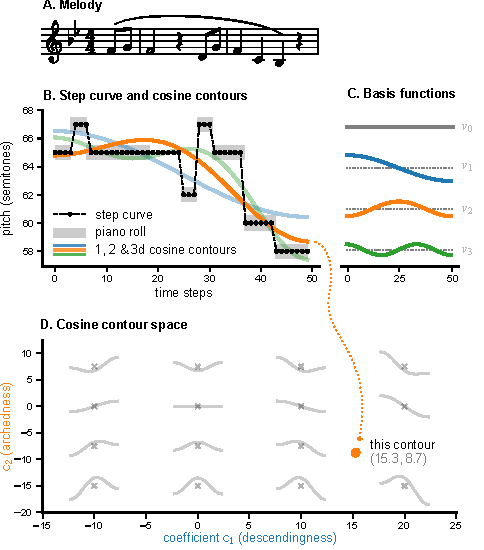
\includegraphics{figs/fig01-cosine-contours.pdf}
    \caption{
        \textbf{Cosine contours} represent a melodic contour as a combination of cosine functions.
        %
        \subfiglabel{(a)}~%
        This is illustrated for a short melodic phrase.
        %
        \subfiglabel{(b)}~%
        A piano roll is interpolated to obtain fixed-length vector of \textsc{midi} pitches (black curve).
        This vector is approximated using a discrete cosine transform (coloured curves).
        Increasing the dimensionality, from, e.g.,~1 (blue) to 3 (green) improves the approximation.
        %
        \subfiglabel{(c)}~%
        The basis functions correspond to simple shapes.
        %
        % \subfiglabel{(d)}~%
        This makes the cosine contour space interpretable, as illustrated in \subfiglabel{(d)} for the first two dimensions. 
        Every point in this space defines a contour shape, varying in what we call the \emph{descendingness} and \emph{archedness}. 
        The orange dot represents the orange contour from \subfiglabel{(b)}.
    }
    \label{fig:representation}
\end{figure}


%—————————————————————————————————
\section{What is melodic contour?}
%—————————————————————————————————


Melodic contour is a general description of a melody's shape that abstracts away from the particular pitches and precise rhythms.
It has been characterised in many different ways.
Ethnomusicologists (and composers) have used \emph{contour typologies}: small sets of contour types \cite{Adams1976}.
David Huron, for example, distinguished nine types of contours by comparing the initial and final pitches to the average pitch on the middle part of a melody \cite{Huron1996}.
When, say, the initial is above the middle, which in turn equals the final, the melody has a `descending-horizontal' contour.
Such a formal typology can be used in \textsc{mir} \cite{Mullensiefen2009}, but typologies have also been defined using verbal descriptions or even drawings \cite{Adams1976,Kelkar2018}.
CantoCore, for example, instructs an annotator to look for six types: ascending, descending, arched, U-shaped, undulating and horizontal \cite{Savage2012}.
Even though the types are less sharply defined, such typologies have inspired cross-cultural generalizations such as the \emph{melodic arch hypothesis}: the claim that melodic phrases tend to be arch-shaped or descending \cite{Huron1996,Savage2015,Tierney2011,Savage2017a}.


In melody extraction from audio, contours are usually represented by sequences of pitches ordered in time.
Various contour features derived from this, such as the range or pitch deviation, have been used in classification tasks \cite{Bittner2017,Panteli2017a,Bittner2015,Salamon2012}.
Contours in symbolic data can be similarly represented as \emph{step curves} (figure \ref{fig:representation}B, black line) \cite{Steinbeck1982,Mullensiefen2012}.
\emph{Parsons code} drastically simplifies a step curve \cite{Parsons1975}.
It describes the direction of movement from one note to the next (up, down, or level) and discards interval size and note durations.
Variants between these two extremes have also been used, by distinguishing various classes of jump sizes \cite{Mullensiefen2004b}.
Another strategy is to focus on salient notes, typically turning points (maxima and minima), and to discard other notes \cite{Adams1976,Steinbeck1982,Salamon2012}.
This often requires special handling of ornaments \cite{Mullensiefen2012}, possibly tailored to the repertoire.
Yet another approach considers the relative ordering of all pairs of notes in a melody, summarized in a matrix.
Such combinatorial models in way expand rather than reduce the representation, break the linearity of the melody and are sensitive to local changes \cite{Mullensiefen2012}.


Finally, one can describe melodies using continuous functions.
Müllensiefen and Wiggins fit a polynomial function to a step curve and use the coefficients to represent the contour \cite{Mullensiefen2012}.
The degree of the polynomial is chosen per phrase, using the Bayesian information criterion (\textsc{bic}) to avoid overfitting.
Polynomial coefficients are quite difficult to interpret, however: they change drastically when the degree changes, and can also be sensitive to changes in the data, especially when the polynomials are not orthogonal and introduce correlations between the coefficients (collinearity).
Instead of fitting a function to the contour, one can also \emph{decompose} the contour and express it as a sum of (orthogonal) basis functions.
Velarde and colleagues have for example used \emph{Haar wavelets} as basis functions in musical pattern discovery \cite{Velarde2016}.
The step-like shapes of those wavelets are well suited to describe particular melodic patterns, but make them less suited for describing the overall contour.
An alternative basis of sinusoidal functions is implicit in Schmuckler's use of a Fourier analyses to represent melodic contour \cite{Schmuckler1999}.
This has been interpreted as measuring the `periodic information' in a melody, and was reported to correlate with perceived similarity.


%—————————————
\section{Data}
%—————————————


With the broad applicability in mind, we analyze music from several independent traditions.
The choice of traditions was partly motivated by our aim to analyze contours at multiple levels of description: we expect (different) regularities at different levels.
At the highest level, complete \emph{songs} can have characteristic shapes, and those shapes may differ between traditions. 
At the smaller level \emph{phrases} may be subject to the melodic arch hypothesis cited above.
Finally, at the smallest level, \emph{melodic motifs} could exhibit sequential structure, for example when melodies in a repertoire are formed by stringing together melodic motifs (sometimes called \emph{centonization} \cite{Nuttall2019}).
We also analyze \emph{random segments} obtained by slicing a melody at random in approximately phrase-length segments, so that their boundaries usually do not overlap with actual phrase boundaries \cite{Cornelissen2020DLfM}.


One tradition for which all of these levels are directly available is Gregorian chant, thanks to two recently released corpora: the CantusCorpus and the GregoBaseCorpus \cite{Cornelissen2020DLfM}.
Gregorian chant has been sung in Roman Catholic churches for well over a thousand years.
The close connection between music and text in chant suggests a natural subdivision of the music into motifs corresponding to words or syllables. 
The notation suggests even smaller motifs: it is based on small figures, called \emph{neumes}, that represent short groups of notes \cite{Kelly2018}.
To analyse motif contours, we use chants from the CantusCorpus (v0.2) with transcriptions of medieval manuscripts, which include neume boundaries. 
We focus on the two largest chant genres: \emph{antiphons} and \emph{responsories}.
Phrase boundaries are not available in the CantusCorpus, however, and so for that, we turn to the GregoBaseCorpus (v0.3) of modern chant transcriptions.
Modern chant notation includes explicit breathing marks (\emph{pausas}), which have been used to extract phrases \cite{Cornelissen2020DLfM}.


Phrase markings are also included in the Essen Folksong Collection \cite{Schaffrath1995}, from which we analyse phrases from German and Chinese folksongs.
We focus on the two largest subsets, `Erk' \cite{Erk1893} (9782 contours) and `Han' (7601 contours).\footnote{%
    %———
    Much is unclear about the exact (bibliographic) origins of the Chinese subset of \emph{Essen}.
    This is problematic given its wide use in computational musicology and deserves further attention from the community.
    }%———
At the level of complete songs, we also add music from the Sioux people made available in the \emph{Densmore Collection} \cite{Densmore1918,Shanahan2014}.
In the supplementary material, we include some further analyses of several other traditions from the \emph{Essen} and \emph{Densmore} collections.


We convert all melodies (be it songs, phrases or motifs) to step contours by extracting note onsets (in quarter notes) and pitches (in \textsc{midi} semitones).
We then interpolate a step function through these points, from which we sample $N=100$ equally spaced pitches.
Those pitches are collected in vectors $\vect x = (x_0, \dots, x_{N-1})$ (black curve in figure \ref{fig:representation}\textsc{a}), which are the basic data analysed in this paper.\footnote{%
    %——
    See \href{https://github.com/bacor/cosine-contours}{github.com/bacor/cosine-contours}
    for data, code and supplements.
    }%——


\begin{figure}[t]
    \centering
    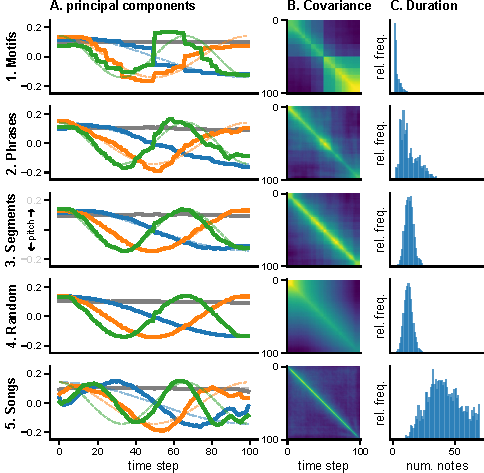
\includegraphics{figs/fig02-pca.pdf}
    \caption{%
        \textbf{Principal components of contours}~%
        %———————————————————————————————————————
        (solid lines) are roughly cosine shaped (dashed) across different levels \textsc{\textbf{(a)}}.
        This is a result of the particular structure of the covariance matrix \textsc{\textbf{(b)}}: matrices of this type have Fourier basis functions as their eigenvectors.
        This is clearest for phrases \textsc{\textbf{(2)}} or random segments from melodies \textsc{\textbf{(3)}}, here of similar length as phrases.
        Crucially, we see the same effect for simulated, contour-like random walks \textsc{\textbf{(4)}}.
        For complete songs \subfiglabel{(5)} the effect is less clear, probably due to differences in typical length \textsc{\textbf{(c)}} and data size.
        Contours in \subfiglabel{1--4} are from Gregorian chant.
    }
    \label{fig:pca}
\end{figure}


Our starting representation makes several assumptions that seem reasonable (and common: \cite{Savage2017a,Tierney2011,Velarde2016}) when only interested in contour.
First, we ignored all rests.
Second, we normalize the duration of all contours.
Both 3-note motifs and 30-note songs are represented by vectors of 100 pitches.
The relative durations within that melody are of course retained, so we would still see that contours of short motives are probably simpler than those of long melodies.
Third, we assume Euclidean distances between melodies.
This is usually problematic, but less so when we are only interested in contour similarity.
Our analyses require that all contours are embedded in a vector space.
Using more sophisticated measures such as dynamic time warping distance, would require us to reconstruct a space (e.g., using multidimensional scaling), and make the analyses less transparent.
Finally, note that we do \emph{not} center the contours to have mean pitch 0.
This is sometimes done to make contours transposition invariant and more directly comparable \cite{Savage2017a,Velarde2016,Cornelissen2020DLfM}.
We will soon see that our proposed representation elegantly resolves this problem without requiring centring.


%———————————————————————————————————————————————————————
\section{Principal components of contours}\label{sec:pc}
%———————————————————————————————————————————————————————


In this section, we explore principal component analysis applied to contours.
The goal of \textsc{pca} is to find a set of orthogonal axes, the \emph{principal components}, that contain most of the variance in the dataset. Note that the principal components, like the original contours from our data, are $N$-dimensional vectors, such that the contours and components can be interpreted and plotted in the same space.


In figure~\ref{fig:pca}\textsc{a}~, we show results from applying \textsc{pca} on a large dataset of Gregorian chant (similar results with German and Chinese folksongs can be found in supplement S2). We plot the first four principal components of several types of melodies: short motifs (syllables), phrases, random segments of melodies, and complete songs.
We show responsory syllables from CantusCorpus for the motifs,
antiphon phrases from the GregoBaseCorpus 
and finally all song contours from GregoBaseCorpus.


Surprisingly, we find that the principal components are highly similar across most of those data sets, and correspond to well-known contour shapes: descending, convex, and—perhaps—undulating. 
This is clearest for the phrases and random segments.
For complete songs the effect is weaker, especially for even smaller datasets (see the supplement S2). 
Besides small data sizes, the fact that songs are
much longer also plays a role (see fig.~\ref{fig:pca}\textsc{c}).
We also applied the analysis on simulated random walks approximating phrases: we draw the number of notes from a similar length distribution, normalize the duration and then sample $N=100$ pitches as before (see supplement S1 for details).
Interestingly, the pattern is now even clearer, suggesting there must be a mathematical explanation.


To give that explanation, we need to first describe \textsc{pca} more formally. We consider a collection of $M$ contour vectors $\vx_m$ of length $N$.
Denote the sample mean by $\bar \vx = \frac{1}{M} \sum_{m} \vx_m$ and the centered data by $\hat \vx_m = \vx_m - \bar \vx$.
The first principal component of the dataset is then defined as a normalized vector $\vu_1 \in \R^D$ for which the projected data $\{\vu_1^T \vx_m: 1 \le m \le M \}$ has maximal variance.
It can be shown (e.g.,~\cite{Jolliffe2002}) that this is the case when $\vu_1$ is an eigenvector corresponding to the largest eigenvalue $\lambda_1$ of the covariance matrix
%———
\begin{align}
    \label{eq:covariance}
    \vS = \frac{1}{M} \sum_{m=1}^M (\vx_m- \bar\vx)(\vx_m - \bar\vx)^T,
\end{align}
%———
so that $\vS \vu_1 = \lambda_1 \vu_1$.
It follows that the projected variance is given by $\lambda_1$, the largest eigenvalue.
The other principal components similarly emerge as the other eigenvectors of the covariance matrix.


The covariance matrices (figure \ref{fig:pca}\textsc{b}) 
for both random walks and our empirical data have a particular structure: they \emph{roughly} resemble \emph{Toeplitz matrices}, which have fixed values along each of their diagonals.
Such covariance structures are frequently encountered in spatial or temporal data, when the covariance decreases with the distance between the points\cite{Gray2006,Novembre2008,Antognini2018}.
With the empirical contours that appears to be the case (and for random walks it is there by design): there is higher correlation between successive pitches and lower correlation between distant pitches.
As a result, the higher covariances are concentrated along the diagonal.
Again, this clearest for the phrases and random segments.
For motifs we see some deviations: two `blocks' in the covariance matrix, and corresponding jumps half way through the principal components.
This is easily explained by the fact that motifs often span only two notes.
In that case, all pitches in the first half of the contour are then perfectly correlated, as are pitches in the final half.
Crucially, despite such deviations from a perfect Toeplitz structure, the principal components are still well-approximated by cosines.


If you let a Toeplitz matrix grow in size, it asymptotically tends towards a \emph{circulant} matrix, preserving properties such as eigenvalues and eigenvectors along the way \cite{Gray2006}.
Circulant matrices have exactly the same values in every row, but rotated one step to the right with respect to the previous row.
This has the surprising result that all circulant matrices have the same eigenvectors: basis vectors of the discrete Fourier transform.
For a real and symmetric matrices, like covariance matrices, this results in cosine-shaped eigenvectors of increasing frequency---exactly what we see in figure \ref{fig:pca}.
We discuss all of this in more detail in the supplement S2.
In sum, because of a Toeplitz-like covariance structure, the principal components of melodic contours will tend to look like cosine functions.


%————————————————————————
\section{Cosine contours}
%————————————————————————

Next we turn this observation, and its explanation, into a proposal for a new contour representation.
The idea is to approximate the principal components by cosine functions and then project the contours on those first few cosines to obtain a low-dimensional representation.
This is exactly equivalent to taking a \emph{discrete cosine transform} (\textsc{dct}) of the contour \cite{Ahmed1974}.


Formally, consider a collection of contours of length $N$ as before.
We approximate the $k$-th principal component $\vu_k$ by a vector $\vect v_k = \bigl(v_k(0), \dots, v_k(N-1)\bigr)$ whose entries are given by the cosine function\footnote{%
    %———
    These basis functions correspond to the most popular version of the discrete cosine transform, \textsc{dct-ii}, for which fast implementations are widely available; others would have been possible \cite{Strang1999}.
    }%———
%———
\begin{align}
    v_k(n) 
        &= \alpha_k \cdot \cos \frac{\pi(2n + 1)k}{2N}.
\end{align}
%———
Here $\alpha_0 = 1/\sqrt{N}$ and $\alpha_k = \sqrt{2/N}$ for $k \ge 1$ are normalizing constants ensuring that $\vect v_k$ has unit norm.
The projection of a contour $\vx = (x_0, \dots, x_{N-1})$ on $\vect v_k$ is then given by the inner product $c_k =  \vect v_k^T \vx$.
Expanding this gives the usual definition of the discrete cosine transform (\textsc{dct-ii}):
%———
\begin{align}
    c_k 
    = \sum_{n=0}^{N-1}
        x_n  \alpha_k \cos \frac{\pi(2n + 1)k}{2N}.
\end{align}
%———
Conversely, the contour can be reconstructed from the coefficients $c_k$ using the inverse transform $x_n = \sum_{k=0}^{N-1} c_k v_k(n)$.
Using only $D<N$ coefficients, we define our low-dimensional \emph{cosine contour representation} as $C_D(\vx) = (c_1, \dots, c_D)$.
Note that we deliberately discard $c_0$.
This coefficient corresponds to a flat line and describes the overall pitch height of a contour: exactly what we need to get rid of to make the contour transposition invariant.
In this way we resolve the centering of contours discussed above.


\begin{figure}[t]
    \centering
    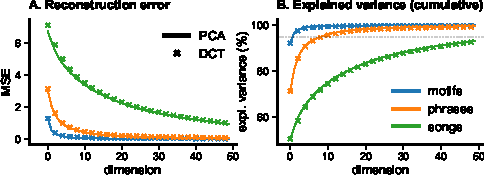
\includegraphics{figs/fig03-evaluation.pdf}
    \caption{%
        \textbf{\textsc{dct} approximates \textsc{pca}},~%
        %——————————————————————————————————————————————
        the optimal transform,
        in terms of the reconstruction error \subfiglabel{(a)} and the explained variance ratio \subfiglabel{(b)}.
        The reconstruction error is the mean squared error between an contour and a lower dimensional reconstruction.
        Note that data corresponds to figure \ref{fig:pca}, and that we did \emph{not} discard the first component $c_0$ of the \textsc{dct} in this figure.
    }
    \label{fig:evaluation}
\end{figure}


Why use this representation instead of principal components?
Indeed, a principal component projection (also known, in this context, as the \emph{Karhunen-Loève transform}), is optimal in several ways \cite{Rao1990,Ahmed1974}.
Not only does it decorrelate the data, it also packs most variance in the first few transform coefficients (sometimes called \emph{energy compaction}), and minimizes the reconstruction error when using only a few coefficients.
However, the transformation depends on the data.
Concretely, the principal components of German phrase contours differ from Chinese ones. 
Any choice for using one of the two is arbitrary. 
In contrast,  the \textsc{dct} is a principled, neutral solution---that approximates the optimal transform.
In fact, the \textsc{dct} was originally introduced for similar reasons \cite{Ahmed1974}, and was then found to empirically approximates \textsc{pca} well in domains ranging from image to audio \cite{Rao1990}.
The current results suggest that the same applies for melodies.


%————————————————————————————————————
\section{Evaluation and case studies}
%————————————————————————————————————


We evaluate proposed contour representation by comparing it to a principal component transformation, to demonstrate that representation is close to the optimum. We further designed three case studies to illustrate its usefulness at the levels of (1) song, (2) phrases and (3) motifs.
The case studies show that the representation is musicologically meaningful, as it allows visualization of variation (1), a quantitative evaluation of constraints on variation (2), and accurate classification into traditional categories (3).
For simplicity, we only look at two dimensional representations in these case studies, but higher dimensions may be useful in practice.


\subsection{Optimality}
%----------------------


To empirically verify the claim that the \textsc{dct} approximates the optimal \textsc{pca} transform, we compute the reconstruction error and the explained variance ratio using the same data as before.
The reconstruction error is measured as the mean square error between a contour and its $D$-dimensional reconstruction, using either the principal components (\textsc{pca}) or cosines (\textsc{dct}) as basis functions (so for $D=N$, the reconstruction is guaranteed to be perfect).
Figure \ref{fig:evaluation}\textsc{a} shows that the reconstruction errors of \textsc{dct} closely approximate that of \textsc{pca}.
For the shorter contours (motifs and phrases), the error very rapidly decreases, indicating that low-dimensional representations are already effective.
Indeed, to explain 95\% of the variance using cosine contours, you need 1 dimension for motifs, 9 for phrases and 61 for songs (this is sometimes called the \emph{effective dimensionality} \cite{Moore2018}).\footnote{%
    %——
    However, note that Moore et al \cite{Moore2018} show that high-dimensional random walks can falsely appear to have a low effective dimensionality.%
    %——
    }


\begin{figure}[t]
    \centering
    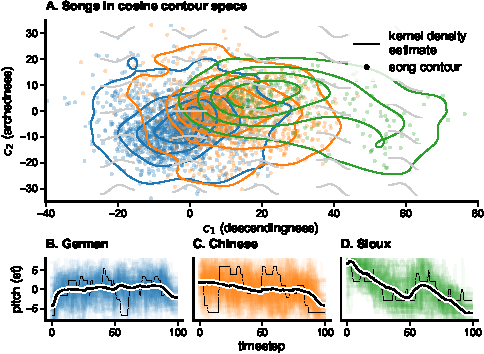
\includegraphics{figs/fig04-songs.pdf}
    \caption{
        \textbf{Songs of three cultures} represented in the cosine contour space \subfiglabel{(a)} show substantial variability.
        The average of all contours in a tradition \subfiglabel{(b--d)} also illustrates this
        (thick black lines; dashed lines highlight one contour).
        }
    \label{fig:songs}
\end{figure}


\subsection{Case Study 1: Visualizing different traditions}
%----------------------------------------------------------


Low dimensional representations of song contours are not likely to be very informative, yet we find that some traditions can be somewhat distinguished in just two dimensions.
Figure \ref{fig:songs} shows song contours from German, Chinese and Sioux songs.
Sioux songs have a striking overall shape (subplot \textsc{d}), often strongly descending, which is reflected in the distribution of contour shapes.
Similarly, German songs appear to be more arch-like than songs from the other traditions.


\subsection{Case Study 2: The melodic arch hypothesis}
%-----------------------------------------------------


In a second case study, we look at the melodic arch hypothesis, which states that \emph{phrases} tend to be arch-shaped or descending \cite{Huron1996} (see figure \ref{fig:melodic-arch}\textsc{a, b}) in a way that it becomes much easier to test (cf.~\cite{Savage2017a}).
We observe that the first component $c_1$ of a cosine representation roughly measures the \emph{descendingness} of the contour, and, similarly, that $-1\cdot c_2$ measures the \emph{archedness}.
The melodic arch hypothesis can thus be reformulated as stating that $c_1$ and $-c_2$ are larger for phrases than %expected by chance.
for random segments of the melodies (cf.~\cite{Cornelissen2020DLfM}).
Comparing Chinese and German phrases, we find that all are significantly ($p \ll 0.001$) more descending and arched than the corresponding random segments (see figure \ref{fig:melodic-arch}\textsc{c, d}).
This demonstrates that the coefficients of the cosine contour representation are musicologically meaningful.


\begin{figure}[t]
    \centering
    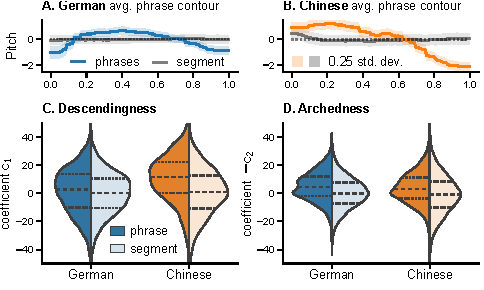
\includegraphics{figs/fig05-melodic-arch.pdf}
    \caption{\textbf{Phrases} of German \subfiglabel{(a)} and Chinese \subfiglabel{(b)} songs tend to be more descending and arched compared to random segments from the same melodies, as visible from their average contours.
    This can be quantified by comparing the first \subfiglabel{(c)} and second \subfiglabel{(d)} coefficients of their cosine representations.}
    \label{fig:melodic-arch}
\end{figure}


\subsection{Case Study 3: Mode classification}
%---------------------------------------------


In the final case study, we evaluate the performance of this contour representation on a task: mode classification in plainchant.
Gregorian chant uses a system of eight \emph{modes}: Dorian, Phrygian, Lydian and Mixolydian, each in the two flavours plagal and authentic.
Modes differ not only in their scales, but also in their melodic movement.
Plagal melodies tend to move lower than authentic ones, closer around the tonal center.
In a recent paper we suggest that the mode of Gregorian chant can be predicted from contours alone, in that case using a Parsons code contour representation \cite{Cornelissen2020ISMIR}.
We sliced up chants in sequences of motifs corresponding to the notational units (so called \emph{neumes}) or textual units: all notes set to one \emph{syllable} of the text would form a unit, and similarly for \emph{words}.
Next, we represented chants as vectors of motif or \emph{term frequencies} (tf), where each entry was weighted by the \emph{inverse document frequency} (df; the number of chants or documents containing that motif).
A linear support vector machine was then trained on these \emph{tf--idf vectors} to predict the mode.


\begin{figure}[t]
    \centering
    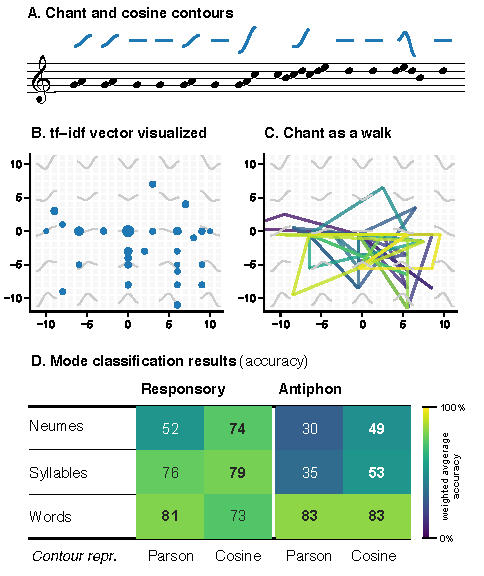
\includegraphics{figs/fig06-mode-classification.pdf}
    \caption{
        \textbf{Motifs used for mode classification} in Gregorian chant. 
        \subfiglabel{(a)}
        A chant is segmented into motifs derived from the notation (neumes) or lyrics (syllables, words).
        The blue curves show the two-dimensional cosine contours for those motifs.
        \subfiglabel{(b)}
        We discretize the contour space and represent the chant as a vector of tf--idf weighed motif frequencies (`grid cell frequencies').
        Dots illustrate the nonzero entries of this vector for the chant shown above.
        \subfiglabel{(c)}
        The chant is now a walk through contour space, but our `bag of motifs` ignores order.
        \subfiglabel{(d)}
        Using these vectors to classify mode, we outperform a previous study using a Parsons code for the smaller motifs neumes and syllables.
        }
    \label{fig:chant}
\end{figure}


We repeat these experiments using a two-dimensional cosine representation for the motifs rather than a Parsons code.
There is one technical problem: whereas cosine contours are continuous, the tf--idf model requires a discrete vocabulary of motifs.
We therefore discretize the cosine contour space to a grid, and effectively treat every chant as a sequence of grid-cells (fig.~\ref{fig:chant}\textsc{c}).
All in all, this introduces two new parameters to the experiment: the dimensionality of the cosine contour and the resolution of the grid.
In this case study, we do not tune these parameters and focus on two dimensional contours, discretized to a grid between $-20$ and $20$ with a grid size of 1.
For ease of reading, the figure~\ref{fig:chant}\textsc{b} shows the grid only from $-10$ to $10$.


The results are summarized in figure \ref{fig:chant}\textsc{d}.
We see an interesting pattern: the cosine contours outperform the original results for small motifs such as neumes and syllables, but not for words, which are much longer motifs. 
This seems to makes sense: two dimensional cosine contours are a fairly crude approximation of those longer contours, but may reasonably approximate short motifs.


%———————————————————————————————————
\section{Discussion and conclusions}
%———————————————————————————————————


This paper proposed a novel representation for melodies using the discrete cosine transform.
Observing that the principal components of melodies tend to be shaped like cosines, this representation approximates the optimal representation in the sense that it packs most variance in a few dimensions.
First, the cosine representation is easily interpretable, since it presents contours as a linear combination of cosine functions with intuitive shapes.
Second, by changing the dimensionality, the level of abstraction of the contour can be varied, allowing arbitrary small reconstruction error by including more and more dimensions.
Third, this representation allows one to map contours at multiple levels, from motifs to songs, to one common space.
The cosine representation thus creates a common ground for comparing contours across traditions and levels.
That is possible as, fourth, the representation is independent of the data, and in that sense culturally neutral.


The observation that principal components of spatial and temporal data can have sinusoidal shapes is not novel, but does not appear to be widely known.
Indeed, the sinusoidal shapes have been interpreted as genuine effects, rather than mathematical artefacts.
For example, one study interpreted gradients in the principal components of human genetic variation across the world as evidence for certain migration events in human history \cite{Cavalli-Sforza1993}.
Closer inspection revealed that those gradients were sinusoidal `artefacts' analogous to those reported in the present paper \cite{Novembre2008}.
Closer to \textsc{mir}, it has been observed that the training trajectories of deep neural networks have sinusoidal principal components \cite{Lorch2016}, for the same reason.
Again, a detailed analysis \cite{Antognini2018} revealed these were artefacts, but accurately reflecting the behaviour of high-dimensional random walks \cite{Antognini2018,Moore2018}. 
We hope this paper helps increasing the awareness of this phenomenon.


The present work only begins to explore this new contour representation and raises many further questions.
One particularly promising possibility is the application to audio data.
We only explored symbolic data, but the proposed representation lends itself well for applications on acoustic data.
One application we hope to explore further is the analysis of speech intonation using the cosine contour representation.
A possible other avenue would be the analysis of folk song recordings, of which vast collections have been collected.
Folk song researchers have often used contour in some way to organize repertoires \cite{Adams1976}, and this representation may contribute to that.
Contour typologies have also be used in cross-cultural comparisons (see e.g.~\cite{Savage2015}).
Many typologies have been proposed \cite{Adams1976,Huron1996,Kelkar2018,Savage2012}, but they have not been systematically evaluated, and we think the proposed representation will be valuable there.


%—————————————————————————
\section{Acknowledgements}
%—————————————————————————


We would like to thank Henkjan Honing and Marianne de Heer Kloots for their feedback on the manuscript.
We would also like to thank the four anonymous reviewers for their careful reviews; we have tried to address all your comments.


%——————————————————————————
\bibliography{bibliography}
%——————————————————————————


\end{document}